\begin{center}
\textbf{\Large Двудольные графы}\\
%\textit{Профи}\\
\textit{06.07.16}
\end{center}

\epigraph{\it Дало две доли провидение \\
На выбор мудрости людской: \\
Или надежду и волнение, \\
Иль безнадежность и покой.}{Е. А. Боратынский, ``Две доли''}

Граф~--- \emph{двудольный,} если его вершины можно раскрасить в~два цвета так, что не~будет рёбер с~концами одинакового цвета.

\begin{problems}
\item
Пусть $\Gamma$~--- двудольный граф с~чёрными и~белыми вершинами.
Докажите, что\\
а) Все циклы в графе $\Gamma$ имеют чётную длину.\\
б) Если в~$\Gamma$ есть замкнутый цикл, проходящий через каждую вершину ровно по~одному разу, то~вершин каждого цвета~--- поровну.\\
в) Если в~$\Gamma$ есть путь, проходящий через каждую вершину ровно по~одному разу, то~число белых вершин отличается от~числа чёрных вершин не~более, чем на~1.

\item Для игры в~классики на~земле нарисован ряд клеток, в~которые вписаны по~порядку числа от~1 до~10, как на~рисунке:

\begin{figure}[h!]
\center{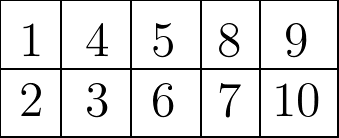
\includegraphics[width=0.3\textwidth]{pic02}}
\end{figure}

Женя прыгнула снаружи в~клетку~1, затем попрыгала по~остальным клеткам (каждый прыжок~--- на~соседнюю по~стороне клетку) и~выпрыгнула наружу из~клетки~10.
Известно, что на~клетке~1 Женя была один~раз, на~клетке~2~--- два~раза, \ldots, на~клетке~9~--- девять~раз.
Сколько раз побывала Женя на~клетке~10?

\item
Замок в~форме треугольника со~стороной 50 метров разбит на~100 треугольных залов со~сторонами $5\,\text{м}$.
В~каждой стенке между залами есть дверь.
Какое наибольшее число залов сможет обойти турист, не~заходя ни~в~какой зал дважды?

%\item а) На~шахматной доске стоят две одинаковых фишки.
%За~один ход можно сдвинуть одну из~фишек на~соседнее поле по~вертикали или горизонтали. Могут~ли фишки перейти в~симметричную относительно средней линии позицию ровно за~2015 ходов?\\
%б) На~шахматной доске стоят пять одинаковых фишек.
%За~один ход можно сдвинуть одну из~фишек на~соседнее поле по~вертикали или горизонтали. Могут~ли фишки перейти в~центрально симметричную позицию ровно за~2015 ходов?

\item а) Докажите, что следующий граф~--- двудольный:
Вершины графа~--- расстановка пары фишек на~шахматной доске. Две расстановки связаны ребром, если позиции0 получаются друг из~друга ходом фишки на~одну клетку по~вертикали или горизонтали.\\
б) На~шахматной доске стоят две одинаковых фишки.
За~один ход можно сдвинуть одну из~фишек на~соседнее поле по~вертикали или горизонтали. Так ходили, пока не~прошли через все возможные позиции. Докажите, что какая-то позиция встретилась не~менее двух раз.

%\item В клетки доски $8\times 8$ записали числа $1, 2,\dots, 64$ в неизвестном порядке. Разрешается узнать сумму чисел в любой паре клеток с общей стороной. Всегда ли можно узнать расположение всех чисел? 
\item а) 10 кружковцев образовали дежурную команду для решения домашних задач. В команде всегда не менее 3 человек. Каждый вечер в команду добавляется один человек либо из неё исключается один человек. Можно ли будет перебрать все допустимые составы команды ровно по одному разу?\\
б) Возможно ли это при другом первоначальном количестве кружковцев?

\item На клетчатой доске $11\times 11$ отмечено 22 клетки так, что на каждой вертикали и на каждой горизонтали отмечено ровно 2 клетки. Два расположения отмеченных клеток эквивалентны, если, меняя любое число раз вертикали между собой и горизонтали между собой, мы из одного расположения можем получить другое. Сколько существует неэквивалентных расположений отмеченных клеток?
\end{problems}
